\documentclass[a4paper]{article}
\usepackage{ctex}
\usepackage[affil-it]{authblk}
\usepackage[backend=bibtex,style=numeric]{biblatex}
\usepackage{amsmath,amsthm,amssymb,amsfonts}
\usepackage{bm}
\usepackage{pifont}
\usepackage{graphicx, subcaption}

\usepackage{geometry}
\geometry{margin=1.5cm, vmargin={0pt,1cm}}
\setlength{\topmargin}{-1cm}
\setlength{\paperheight}{29.7cm}
\setlength{\textheight}{25.3cm}

\addbibresource{citation.bib}

\begin{document}
% =================================================
\title{有限元方法 2025 秋冬作业三}

\author{曾申昊 3220100701
  \thanks{邮箱: \texttt{3097714673@qq.com}
                            \texttt{或} \texttt{3220100701@zju.edu.cn}}}
\affil{电子科学与技术 2202,浙江大学 }


\date{更新时间: \today}

\maketitle


% ============================================
\section*{1. 二阶 Sobolev 空间 $H^2(0,1)$}

\begin{enumerate}
    \item[(a)] 依次验证内积的三条准则:
            \begin{itemize}
                \item $(u+w,v)_{H^2}=(u,v)_{H^2}+(w,v)_{H^2}$ 且 $(\lambda u,v)_{H^2}=\lambda (u,v)_{H^2}$
                \item $(u,v)_{H^2}=\displaystyle\int_{0}^{1}(uv+u'v'+u''v'')\text{d}x=(v,u)_{H^2}$
                \item $(u,u)_{H^2}=\displaystyle\int_{0}^{1}\left(u^2+(u')^2+(u'')^2\right)\text{d}x\geq 0$,
                        当且仅当 $u=0$ 时等号成立
            \end{itemize}
            因此 $(\bullet, \bullet)_{H^2}$ 是一个内积。
    \item[(b)] 由内积 $(\bullet, \bullet)_{H^2}$ 诱导的范数为 
            \begin{equation}
                \Vert u\Vert_{H^2}=\sqrt{(u,u)_{H^2}}
                =\sqrt{\int_{0}^{1}\left(u^2+(u')^2+(u'')^2\right)\text{d}x}
                =\sqrt{\Vert u\Vert_{L^2}^2+\Vert u'\Vert_{L^2}^2+\Vert u''\Vert_{L^2}^2}
            \end{equation}
            对于 $H^2(0,1)$ 中的任意 Cauchy 列 
            $\{u_n\}$有,对 $\forall \varepsilon>0$,
            $\exists N_0 \in \mathbb{N}$,当 $m,n>N_0$ 时有
            \begin{equation}
                \Vert u_n-u_m\Vert_{H^2} < \varepsilon
            \end{equation}
            也就是
            \begin{equation}
                \Vert u_n-u_m\Vert_{L^2}^2+\Vert u_n'-u_m'\Vert_{L^2}^2+\Vert u_n''-u_m''\Vert_{L^2}^2 < \varepsilon^2
            \end{equation}
            由 $L^2(0,1)$ 的完备性可知 $\{u_n\}$、$\{u_n'\}$ 和 $\{u_n''\}$ 
            在 $L^2$ 范数意义下分别收敛于 $u$、$v$ 和 $w$。
            我们接下来需要证明 $u' \overset{a.e.}{=} v$ 以及 $v' \overset{a.e.}{=} w$。
            \begin{equation}
                \begin{aligned}
                    \int_{0}^{1}|u_n'-v|\text{d}x
                    &\leq \sqrt{\int_{0}^{1}(u_n'-v)^2\text{d}x}
                    \sqrt{\int_{0}^{1}1^2\text{d}x}\\
                    &=\Vert u_n'-v \Vert_{L^2} \rightarrow 0
                \end{aligned}
            \end{equation}
            由 Fatou 引理可知
            \begin{equation}
                \begin{aligned}
                    \int_{0}^{1}|u'-v|\text{d}x
                    &=\int_{0}^{1}\lim_{n\rightarrow \infty}|u_n'-v|\text{d}x\\
                    &\leq \liminf_{n\rightarrow \infty}\int_{0}^{1}|u_n'-v|\text{d}x=0
                \end{aligned}
            \end{equation}
            由此可得 $u' \overset{a.e.}{=} v$,同理可得 $v' \overset{a.e.}{=} w$,
            因此 $u\in H^2(0,1)$。最后易证 $\Vert u_n-u\Vert_{H^2} \rightarrow 0$,
            综上我们证明了 $H^2(0,1)$ 是一个 Hilbert 空间。
    \item[(c)] 由于 $v'\in \text{AC}[0,1]$,我们有
            \begin{equation}
                u'(x) = u'(a) + \int_{a}^{x}u''(t)\text{d}t
            \end{equation}
            令 $F(s)=\int_{a}^{s}u''(t)\text{d}t$,等式两边积分可得
            \begin{gather}
                \int_{a}^{x}u'(s)\text{d}s = \int_{a}^{x}u'(a)\text{d}s + \int_{a}^{x}F(s)\text{d}s\\
                u(x)-u(a) = u'(a)(x-a) + \int_{a}^{x}F(s)\text{d}s\\
                u(x)-u(a) = u'(a)(x-a) + 
                sF(s)\Big|_{s=a}^{s=x} - \int_{a}^{x}sF'(s)\text{d}s\\
                u(x)-u(a) = u'(a)(x-a) + 
                x\int_{a}^{x}u''(s)\text{d}s- \int_{a}^{x}su''(s)\text{d}s
            \end{gather}
            整理后可得结论。
\end{enumerate}

\section*{2. 区间 $[0,1]$ 上的分段 Lagrange 插值}

\begin{enumerate}
    \item[(a)] 由第 1 题的 (c) 小问可知
            \begin{equation}
                u(x) = u(x_i) + u'(x_i)(x-x_i) + r(x)
                \qquad x\in [x_i, x_{i+1}]
            \end{equation}
            其中 $r(x)=\int_{x_i}^{x}u''(t)(x-t)\text{d}t$。
            \begin{equation}
                \begin{aligned}
                    (I_h u)(x) &= u(x_i) + u'(x_i)(x-x_i) + (I_h r)(x)\\
                               &= u(x_i) + u'(x_i)(x-x_i) + r(x_{i+1})\frac{x-x_i}{h_i}\\
                \end{aligned}
                \qquad x\in [x_i, x_{i+1}]
            \end{equation}
            其中 $h_i=x_{i+1}-x_i$,然后可以进行误差估计
            \begin{equation}
                \begin{aligned}
                    \Vert u-I_h u \Vert_{L^{\infty}(x_i,x_{i+1})} 
                    &= \max_{x\in [x_i,x_{i+1}]}|r(x)- (I_h r)(x)|\\
                    &= \max_{x\in [x_i,x_{i+1}]}\left|\int_{x_i}^{x}u''(t)(x-t)\text{d}t
                    -\frac{x-x_i}{h_i}\int_{x_i}^{x_{i+1}}u''(t)(x_{i+1}-t)\text{d}
                    \right|\\
                    &\leq \max_{x\in [x_i,x_{i+1}]}\left\{
                        \left|\int_{x_i}^{x}u''(t)(x-t)\text{d}t\right|
                        +\left|\frac{x-x_i}{h_i}\int_{x_i}^{x_{i+1}}
                        {u''(t)(x_{i+1}-t)\text{d}t}\right|
                    \right\}\\
                    &\leq \Vert u''\Vert_{L^{\infty}(x_i,x_{i+1})} \max_{x\in [x_i,x_{i+1}]}\left\{
                        \left|\int_{x_i}^{x}(x-t)\text{d}t\right|
                        +\left|\frac{x-x_i}{h_i}\int_{x_i}^{x_{i+1}}
                        {(x_{i+1}-t)\text{d}t}\right|
                    \right\}\\
                    &=\Vert u''\Vert_{L^{\infty}(x_i,x_{i+1})} \max_{x\in [x_i,x_{i+1}]}\left\{
                        \left|\frac{(x-x_i)^2}{2}\right|
                        +\left|\frac{x-x_i}{h_i}\frac{h_i^2}{2}\right|
                    \right\}\\
                    &\leq h_i^2 \Vert u''\Vert_{L^{\infty}(x_i,x_{i+1})}
                \end{aligned}
            \end{equation}
            \begin{equation}
                \begin{aligned}
                    \Vert u'-(I_h u)' \Vert_{L^{\infty}(x_i,x_{i+1})} 
                    &= \max_{x\in [x_i,x_{i+1}]}\left|r'(x)- (I_h r)'(x)\right|\\
                    &= \max_{x\in [x_i,x_{i+1}]}\left|\int_{x_i}^{x}u''(t)\text{d}t-\frac{r(x_{i+1})}{h_i}\right|\\
                    &\leq \max_{x\in [x_i,x_{i+1}]}\left\{
                        \left|\int_{x_i}^{x}u''(t)\text{d}t\right|
                        +\left|\frac{1}{h_i}\int_{x_i}^{x_{i+1}}u''(t)(x_{i+1}-t)\text{d}t\right|
                    \right\}\\
                    &\leq \Vert u''\Vert_{L^{\infty}(x_i,x_{i+1})} \max_{x\in [x_i,x_{i+1}]}\left\{
                        \left|\int_{x_i}^{x}1\text{d}t\right|
                    +\left|\frac{1}{h_i}\int_{x_i}^{x_{i+1}}(x_{i+1}-t)\text{d}t\right|
                    \right\}\\
                    &= \frac{3h_i}{2} \Vert u''\Vert_{L^{\infty}(x_i,x_{i+1})}
                \end{aligned}
            \end{equation}
            上述两式控制了区间 $[x_i,x_{i+1}]$ 上的误差,取各子区间最大值即得整体误差估计。
    \item[(b)] 将每个子区间 $[x_i, x_{i+1}]$ 划分成两个等长的子区间,令其中点为
            \begin{equation}
                m_i = \frac{x_i+x_{i+1}}{2} \qquad i=0,1,\ldots,N
            \end{equation}
            在每组相邻节点 $\{x_i, m_i, x_{i+1}\}$ 上构造二次插值多项式
            \begin{equation}
                (I_h f)(x) = f(x_i)L_{i,0}(x) + f(m_i)L_{i,1}(x) + f(x_{i+1})L_{i,2}(x)
                \qquad x\in [x_i, x_{i+1}]
            \end{equation}
            其中
            \begin{align}
                L_{i,0}(x) &= \frac{(x-m_i)(x-x_{i+1}){}}{(x_i-m_i)(x_i-x_{i+1})}\\
                L_{i,1}(x) &= \frac{(x-x_i)(x-x_{i+1}){}}{(m_i-x_i)( m_i-x_{i+1})}\\
                L_{i,2}(x) &= \frac{(x-x_i)(x-m_i)}{(x_{i+1}-x_i)(x_{i+1}-m_i)}
            \end{align}
    \item[(c)] 类似 (a) 小问,作 $u(x)$ 的泰勒展开
            \begin{equation}
                u(x) = u(x_i) + u'(x_i)(x-x_i) + \frac{u''(x_i)}{2}(x-x_i)^2 + r(x)
                \qquad x\in [x_i, x_{i+1}]
            \end{equation}
            其中 $r(x)=\frac{1}{2}\int_{x_i}^{x}u'''(t)(x-t)^2\text{d}t$。
            \begin{equation}
                \begin{aligned}
                    (I_h u)(x) = \ &u(x_i) + u'(x_i)(x-x_i) + \frac{u''(x_i)}{2}(x-x_i)^2 + (I_h r)(x)\\
                               = \ &u(x_i) + u'(x_i)(x-x_i) + \frac{u''(x_i)}{2}(x-x_i)^2\\ 
                               &+ r(m_i)\frac{(x-x_i)(x-x_{i+1})}{(m_i-x_i)(m_i-x_{i+1})}
                               + r(x_{i+1})\frac{(x-x_i)(x-m_i)}{(x_{i+1}-x_i)(x_{i+1}-m_i)}
                \end{aligned}
                \qquad x\in [x_i, x_{i+1}]
            \end{equation}
            然后可以进行误差估计
            \begin{equation}
                \begin{aligned}
                    |r(x)| &\leq \frac{1}{2}\int_{x_i}^{x}|u'''(t)|(x-t)^2\text{d}t\\
                    &\leq \frac{1}{2} \sqrt{\int_{x_i}^{x}|u'''(t)|^2\text{d}t \int_{x_i}^{x}(x-t)^4\text{d}t}\\
                    &\leq \frac{1}{2} \Vert u''' \Vert_{L^2(x_i,x_{i+1})} \sqrt{\int_{x_i}^{x}(x-t)^4\text{d}t}\\
                    &\leq \frac{1}{2\sqrt{5}} h_i^{\frac{5}{2}} \Vert u''' \Vert_{L^2(x_i,x_{i+1})}\\
                \end{aligned}
            \end{equation}
            \begin{equation}
                \begin{aligned}
                    \Vert u-I_h u \Vert_{L^2(x_i,x_{i+1})}
                    &= \sqrt{\int_{x_i}^{x_{i+1}}|r(x)- (I_h r)(x)|^2\text{d}x}\\
                    &\leq \sqrt{\int_{x_i}^{x_{i+1}}\big(
                        |r(x)| + |r(m_i)L_{i,1}(x)|
                        + |r(x_{i+1})L_{i,2}(x)|
                    \big)^2\text{d}x}\\
                    &\leq \Vert u''' \Vert_{L^2(x_i,x_{i+1})} 
                    \sqrt{\int_{x_i}^{x_{i+1}}\frac{1}{20}h_i^5\big(
                        1 + |L_{i,1}(x)|
                        + |L_{i,2}(x)|
                    \big)^2\text{d}x}\\
                    &\leq C_1 h_i^3 \Vert u''' \Vert_{L^2(x_i,x_{i+1})}
                \end{aligned}
            \end{equation}
            \begin{equation}
                \begin{aligned}
                    |r'(x)| &\leq \int_{x_i}^{x}|u'''(t)||(x-t)|\text{d}t\\
                    &\leq \sqrt{\int_{x_i}^{x}|u'''(t)|^2\text{d}t \int_{x_i}^{x}(x-t)^2\text{d}t}\\
                    &\leq \Vert u''' \Vert_{L^2(x_i,x_{i+1})} \sqrt{\int_{x_i}^{x}(x-t)^2\text{d}t}\\
                    &\leq \frac{1}{2\sqrt{3}} h_i^{\frac{3}{2}} \Vert u''' \Vert_{L^2(x_i,x_{i+1})}\\
                \end{aligned}
            \end{equation}
            \begin{equation}
                \begin{aligned}
                    \Vert u'-(I_h u)' \Vert_{L^2(x_i,x_{i+1})}
                    &= \sqrt{\int_{x_i}^{x_{i+1}}|r'(x)- (I_h r)'(x)|^2\text{d}x}\\
                    &\leq \sqrt{\int_{x_i}^{x_{i+1}}\big(
                        |r'(x)| + |r(m_i)L_{i,1}'(x)|
                        + |r(x_{i+1})L_{i,2}'(x)|
                    \big)^2\text{d}x}\\
                    &\leq \Vert u''' \Vert_{L^2(x_i,x_{i+1})} 
                    \sqrt{\int_{x_i}^{x_{i+1}}\frac{1}{12}h_i^3\big(
                        1 + |L_{i,1}'(x)|
                        + |L_{i,2}'(x)|
                    \big)^2\text{d}x}\\
                    &\leq C_2 h_i^2 \Vert u''' \Vert_{L^2(x_i,x_{i+1})}
                \end{aligned}
            \end{equation}
            类似的,取各子区间最大值即得整体误差估计。
\end{enumerate}

\section*{3. 区间 $[0,1]$ 上两点边值问题的有限元方法}

\begin{enumerate}
    \item[(a)] 范数 $\Vert\bullet\Vert_{H^1(0,1)}$, $\Vert\bullet\Vert_{H^2(0,1)}$ 
                和半范数 $|\bullet|_{H^2(0,1)}$, $|\bullet|_{H^3(0,1)}$ 的定义如下
            \begin{equation}
                \Vert u \Vert_{H^1(0,1)}
                =\left(
                    \sum_{|\alpha|\leq 1} \Vert\partial^\alpha u\Vert^2_{L^2(0,1)}
                \right)^{\frac{1}{2}}
                =\sqrt{\Vert u\Vert^2_{L^2(0,1)}
                    +\Vert u'\Vert^2_{L^2(0,1)}}
            \end{equation}
            \begin{equation}
                \Vert u \Vert_{H^2(0,1)}
                =\left(
                    \sum_{|\alpha|\leq 2} \Vert\partial^\alpha u\Vert^2_{L^2(0,1)}
                \right)^{\frac{1}{2}}
                =\sqrt{\Vert u\Vert^2_{L^2(0,1)}
                    +\Vert u'\Vert^2_{L^2(0,1)}
                    +\Vert u''\Vert^2_{L^2(0,1)}}
            \end{equation}
            \begin{equation}
                |u|_{H^2(0,1)}
                =\left(
                    \sum_{|\alpha|= 2} \Vert\partial^\alpha u\Vert^2_{L^2(0,1)}
                \right)^{\frac{1}{2}}
                =\Vert u''\Vert_{L^2(0,1)}
            \end{equation}
            \begin{equation}
                |u|_{H^3(0,1)}
                =\left(
                    \sum_{|\alpha|= 3} \Vert\partial^\alpha u\Vert^2_{L^2(0,1)}
                \right)^{\frac{1}{2}}
                =\Vert u'''\Vert_{L^2(0,1)}
            \end{equation}
    \item[(b)] 该问题的有限元方法可以由以下推导得到
    \begin{equation}
        \begin{gathered}
            -\int_{0}^{1}(au')'v\text{d}x + 2\int_{0}^{1}uv\text{d}x = \int_{0}^{1}fv\text{d}x \\
            -\Big.au'v\Big|_0^1+\int_{0}^{1}au'v'\text{d}x + 2\int_{0}^{1}uv\text{d}x = \int_{0}^{1}fv\text{d}x \\
            \int_{0}^{1}au'v'\text{d}x + 2\int_{0}^{1}uv\text{d}x = \int_{0}^{1}fv\text{d}x \\
        \end{gathered}
    \end{equation}
    取 $v_h \in V_h$,分段一次有限元空间定义如下
    \begin{equation}
        \begin{aligned}
            V_h&=\left\{
                v_h\in C[0,1] : v_h|_{[x_i,x_{i+1}]}\in P_1(x_i,x_{i+1}), v_h(0)=0
            \right\}\\
            &=span\{\phi_1, \phi_2, \ldots, \phi_N\}
        \end{aligned}
    \end{equation}
    其中 $\phi_i$ 是节点 $x_i$ 处的分段一次基函数:
    \begin{equation}
        \phi_i(x) = \begin{cases}
            \displaystyle\frac{x-x_{i-1}}{x_i-x_{i-1}} \quad & x\in [x_{i-1}, x_i] \\
            \displaystyle\frac{x_{i+1}-x}{x_{i+1}-x_i} & x\in [x_i, x_{i+1}] \\
            0 & \text{else}
        \end{cases}
    \end{equation}
    误差估计由第 2 题的 (a) 小问易得
    \begin{equation}
        \Vert u-u_h \Vert_{L^2(0,1)} \leq C_1 h^2 \Vert u'' \Vert_{L^2(0,1)}
        = C_1 h^2 |u|_{H^2(0,1)}
    \end{equation}
    \begin{equation}
        \Vert u-u_h \Vert_{H^1(0,1)}
        = \Vert u'-u_h' \Vert^2_{L^2(0,1)}
        \leq C_2 h \Vert u'' \Vert_{L^2(0,1)}
        = C_2 h |u|_{H^2(0,1)}
    \end{equation}
    \item[(c)] 该问题的有限元方法由 (b) 小问已经得到,
            其分段二次有限元空间定义如下
            \begin{equation}
                \begin{aligned}
                    V_h&=\left\{
                        v_h\in C[0,1] : v_h|_{[x_i,x_{i+1}]}\in P_2(x_i,x_{i+1}), v_h(0)=0
                    \right\}\\
                    &=span\{\phi_1, \phi_2, \ldots, \phi_{2N+1}\}
                \end{aligned}
            \end{equation}
            其中 $\phi_i$ 是节点 $x_i$ 和中点 $m_i$ 处的分段二次基函数:
            \begin{equation}
                \phi_{2i}(x) = \begin{cases}
                    \displaystyle\frac{(x-x_{i-1})(x-m_{i-1})}{(x_i-x_{i-1})(x_i-m_{i-1})} \quad & x\in [x_{i-1}, x_i] \\
                    \displaystyle\frac{(x-x_{i+1})(x-m_i)}{(x_i-x_{i+1})(x_i-m_i)} & x\in [x_i, x_{i+1}] \\
                    0 & \text{else}
                \end{cases}
                \qquad i=1,2,\ldots,N
            \end{equation}
            \begin{equation}
                \phi_{2i+1}(x) = \begin{cases}
                    \displaystyle\frac{(x-x_{i})(x-x_{i+1})}{(m_i-x_{i})(m_i-x_{i+1})} & x\in [x_i, x_{i+1}] \\
                    0 & \text{else}
                \end{cases}
                \qquad i=0,1,\ldots,N
            \end{equation}
            其中 $m_i=\frac{x_i+x_{i+1}}{2}$。
            误差估计由第 2 题的 (c) 小问易得
            \begin{equation}
                \Vert u-u_h \Vert_{L^2(0,1)} \leq C_1 h^3 \Vert u''' \Vert_{L^2(0,1)}
                = C_1 h^3 |u|_{H^3(0,1)}
            \end{equation}
            \begin{equation}
                \Vert u-u_h \Vert_{H^1(0,1)}
                = \Vert u'-u_h' \Vert^2_{L^2(0,1)}
                \leq C_2 h^2 \Vert u''' \Vert_{L^2(0,1)}
                = C_2 h^2 |u|_{H^3(0,1)}
            \end{equation}
\end{enumerate}

\section*{4. 区间 $[0,1]$ 上两点边值问题的数值方法}

\begin{enumerate}
    \item[(a)] 记 $h=\frac{1}{N+1}$,该问题的分段一次有限元方法为
            \begin{equation}
                \int_{0}^{1} u_h' v_h' \text{d}x = \int_{0}^{1} f v_h \text{d}x \qquad \forall v_h\in H_0^1(0,1)
                \label{分段一次有限元问题}
            \end{equation}
            设 $u_h=\sum_{i=1}^{N}u_i\phi_i$,其中 $\phi_i$ 是节点 $x_i$ 处的分段一次基函数:
            \begin{equation}
                \phi_i(x) = \begin{cases}
                    \displaystyle\frac{x-x_{i-1}}{h} \quad & x\in [x_{i-1}, x_i] \\
                    \displaystyle\frac{x_{i+1}-x}{h} & x\in [x_i, x_{i+1}] \\
                    0 & \text{else}
                \end{cases}
            \end{equation}
            将其代入式 (\ref{分段一次有限元问题}) 计算可得有限元矩阵
            $A_{\text{FEM}} \in \mathbb{R}^{N\times N}$
            \begin{equation}
                A_{\text{FEM}} =
                \begin{pmatrix}
                    \frac{2}{h} & -\frac{1}{h} & 0 & \cdots & \cdots & 0\\
                    -\frac{1}{h} & \frac{2}{h} & -\frac{1}{h} & \cdots & \cdots & 0\\
                    0 & -\frac{1}{h} & \frac{2}{h} & \ddots & \cdots & 0\\
                    \vdots & \vdots & \ddots & \ddots & \ddots & \vdots\\
                    \vdots & \vdots & \vdots & -\frac{1}{h} & \frac{2}{h} & -\frac{1}{h}\\
                    0 & 0 & 0 & \cdots & -\frac{1}{h} & \frac{2}{h}
                \end{pmatrix}
            \end{equation}
            该问题的有限差分方法为
            \begin{equation}
                -\frac{u_{i+1}-2u_i+u_{i-1}}{h^2} = f(x_i)
                \qquad i=1,2,\ldots,N
            \end{equation}
            计算可得有限差分矩阵
            $A_{\text{FDM}} \in \mathbb{R}^{N\times N}$
            \begin{equation}
                A_{\text{FDM}} = 
                \begin{pmatrix}
                    \frac{2}{h^2} & -\frac{1}{h^2} & 0 & \cdots & \cdots & 0\\
                    -\frac{1}{h^2} & \frac{2}{h^2} & -\frac{1}{h^2} & \cdots & \cdots & 0\\
                    0 & -\frac{1}{h^2} & \frac{2}{h^2} & \ddots & \cdots & 0\\
                    \vdots & \vdots & \ddots & \ddots & \ddots & \vdots\\
                    \vdots & \vdots & \vdots & -\frac{1}{h^2} & \frac{2}{h^2} & -\frac{1}{h^2}\\
                    0 & 0 & 0 & \cdots & -\frac{1}{h^2} & \frac{2}{h^2}
                \end{pmatrix}
            \end{equation}
            可以发现这两个仅仅差一个常数倍。
    \item[(b)] 设 $u_h=\sum_{i=1}^{2N+1}u_i\phi_i$,
                其中 $\phi_i$ 是节点 $x_i$ 和中点 $m_i$ 处的分段二次基函数:
            \begin{equation}
                \phi_{2i}(x) = \begin{cases}
                    \displaystyle\frac{2(x-x_{i-1})(x-m_{i-1})}{h^2} \quad & x\in [x_{i-1}, x_i] \\
                    \displaystyle\frac{2(x-x_{i+1})(x-m_i)}{h^2} & x\in [x_i, x_{i+1}] \\
                    0 & \text{else}
                \end{cases}
                \qquad i=1,2,\ldots,N
            \end{equation}
            \begin{equation}
                \phi_{2i+1}(x) = \begin{cases}
                    \displaystyle\frac{4(x-x_{i})(x-x_{i+1})}{h^2} & x\in [x_i, x_{i+1}] \\
                    0 & \text{else}
                \end{cases}
                \qquad i=0,1,\ldots,N
            \end{equation}
            将其代入式 (\ref{分段一次有限元问题}) 计算可得有限元矩阵
            $A_{\text{FEM}} \in \mathbb{R}^{(2N+1)\times (2N+1)}$
            \begin{equation}
                A_{\text{FEM}} =
                \begin{pmatrix}
                    \frac{16}{3h} & \frac{8}{3h} & 0 & 0 & \cdots & \cdots & 0\\
                    \frac{8}{3h} & \frac{14}{3h} & \frac{8}{3h} & \frac{1}{3h} & \cdots & \cdots & 0\\
                    0 & \frac{8}{3h} & \frac{16}{3h}  & \frac{8}{3h} & \cdots & \cdots & 0\\
                    0 & \frac{1}{3h} & \frac{8}{3h} & \frac{14}{3h} & \ddots & \cdots & 0\\
                    \vdots & \vdots & \vdots & \ddots & \ddots & \ddots & \vdots\\
                    \vdots & \vdots & \vdots & \vdots & \frac{8}{3h} & \frac{14}{3h} & \frac{8}{3h}\\
                    0 & 0 & 0 & 0 & \cdots & \frac{8}{3h} & \frac{16}{3h}
                \end{pmatrix}
            \end{equation}
            在分段二次有限元问题中,我们添加中点加细了网格。在高阶有限差分中,
            或许可以利用中点构造具有更高收敛阶的差分格式,来拟合二阶导数。
\end{enumerate}

\section*{5. 格林函数 $G(\bullet, y)\in H^1_0(0,1)$}

\begin{enumerate}
    \item[(a)] 将 $\frac{\partial G}{\partial x}(x,y)$ 代入方程可得
            \begin{equation}
                \frac{\partial G}{\partial x}(x,y)=\begin{cases}
                    1-y, & x<y \\
                    -y, & x>y
                \end{cases}
            \end{equation}
            \begin{equation}
                \begin{aligned}
                    \int_{0}^{1}v'(x)\frac{\partial G}{\partial x}(x,y)\text{d}x
                    &= \int_{0}^{y}v'(x)\frac{\partial G}{\partial x}(x,y)\text{d}x
                    + \int_{y}^{1}v'(x)\frac{\partial G}{\partial x}(x,y)\text{d}x\\
                    &= \int_{0}^{y}v'(x)(1-y)\text{d}x
                    + \int_{y}^{1}v'(x)(-y)\text{d}x\\
                    &= \left(v(y)-v(0)\right)(1-y)
                    + \left(v(1)-v(y)\right)(-y)\\
                    &=v(y)
                \end{aligned}
            \end{equation}
            $G(x,y)$ 是该问题的解。
    \item[(b)] 交换 $x$ 和 $y$ 可得
            \begin{equation}
                \begin{aligned}
                    G(y,x)&=\begin{cases}
                        (1-x)y, & y<x \\
                        x(1-y), & y>x
                    \end{cases}\\
                    &=\begin{cases}
                        (1-y)x, & x<y \\
                        y(1-x), & x>y
                    \end{cases}=G(x,y)
                \end{aligned}
            \end{equation}
            要证明该函数是 $-u''=f$ 的格林函数,即证明 $-\frac{\partial^2 G}{\partial x^2}(x,y)=\delta(x-y)$。
            \begin{equation}
                \begin{cases}
                    \displaystyle\int_{0}^{1}-\frac{\partial^2 G}{\partial x^2}(x,y)\text{d}x=
                    \left.-\frac{\partial G}{\partial x}(x,y)\right|_{x=0}^{x=1}
                    =(-y)-(1-y)=1\\
                    \displaystyle\int_{0}^{1}\delta(x-y)\text{d}x=1
                \end{cases}
            \end{equation}
        \item[(c)] 通过分部积分可证明结论 
            \begin{equation}
                \begin{aligned}
                    \int_{0}^{1}G(x,y)f(y)\text{d}y
                    &=-\int_{0}^{1}G(x,y)u''(y)\text{d}y\\
                    &=-\Big.G(x,y)u'(y)\Big|_{y=0}^{y=1}
                    +\int_{0}^{1}\frac{\partial G}{\partial y}(x,y)u'(y)\text{d}y\\
                    &=-G(x,1)u'(1)+G(x,0)u'(0) + u(x)\\
                    &=u(x)
                \end{aligned}
            \end{equation}
            倒数第二个等号成立由 (a) 结论可得;最后一个等号成立是由于$G(x,1)=G(x,0)=0$。
\end{enumerate}

\section*{6. 分片一次的有限元方法编程}

\begin{enumerate}
    \item[(a)] 取 $h=0.25$,其网格剖分图像如图 \ref{$h=0.25$网格剖分图像} 所示
                \begin{figure}[htbp]
                    \centering
                    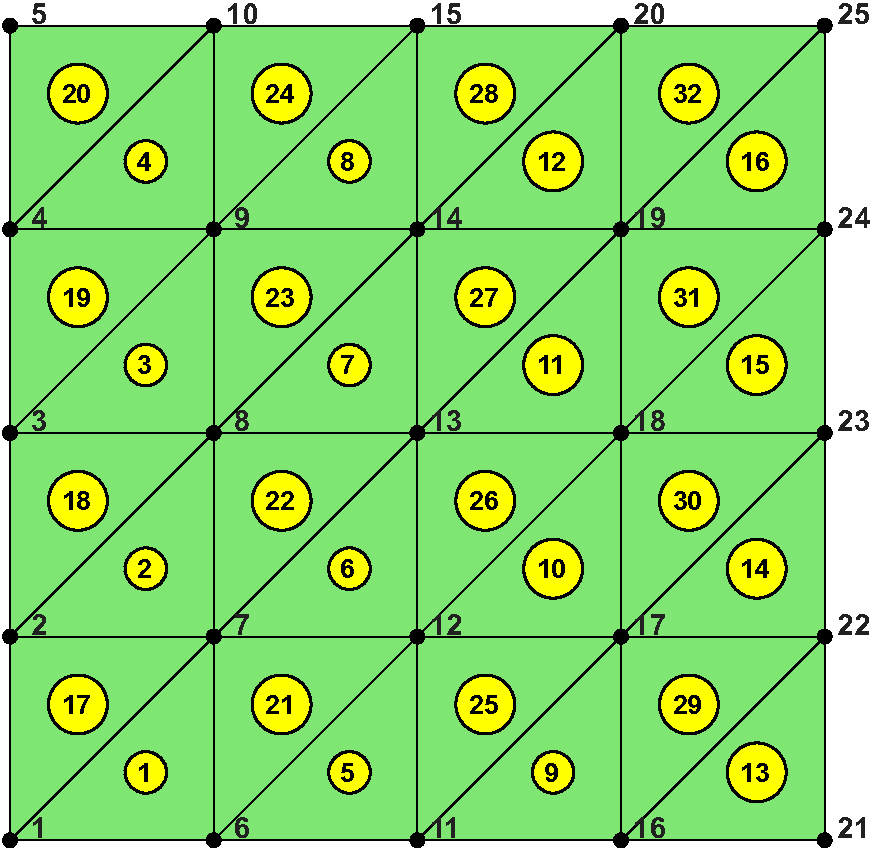
\includegraphics[width=0.4\textwidth]
                        {../../Programming/Linear Finite Element Methods/image/mesh.pdf}
                    \caption{$h=0.25$网格剖分图像}
                    \label{$h=0.25$网格剖分图像}
                \end{figure}
    \item[(b)] 当 $h=0.25$ 和 $h=0.125$ 时, $u_h$ 的图像
                分别如图 \ref{$h=0.25$ 时 $u_h$ 的图像}
                和图 \ref{$h=0.125$ 时 $u_h$ 的图像} 所示
                \begin{figure}[htbp]
                    \centering
                    \begin{subfigure}{0.4\textwidth}
                        \centering
                        
\includegraphics[width=\textwidth]
                            {../../Programming/Linear Finite Element Methods/image/pic1FEM_0.25.pdf}
                    \end{subfigure}
                    \begin{subfigure}{0.4\textwidth}
                        \centering
                        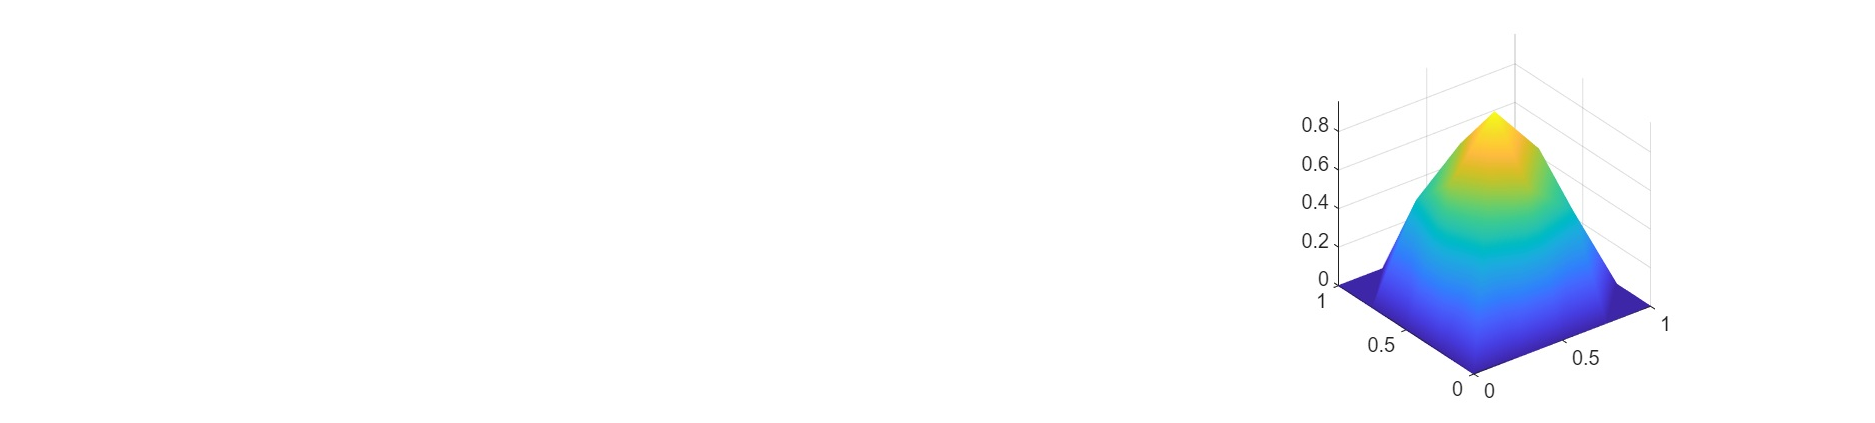
\includegraphics[width=\textwidth]
                            {../../Programming/Linear Finite Element Methods/image/pic2FEM_0.25.pdf}
                    \end{subfigure}
                    \caption{$h=0.25$ 时 $u_h$ 的图像}
                    \label{$h=0.25$ 时 $u_h$ 的图像}
                \end{figure}
                \begin{figure}
                    \centering
                    \begin{subfigure}{0.4\textwidth}
                        \centering
                        
\includegraphics[width=\textwidth]
                            {../../Programming/Linear Finite Element Methods/image/pic1FEM_0.125.pdf}
                    \end{subfigure}
                    \begin{subfigure}{0.4\textwidth}
                        \centering
                        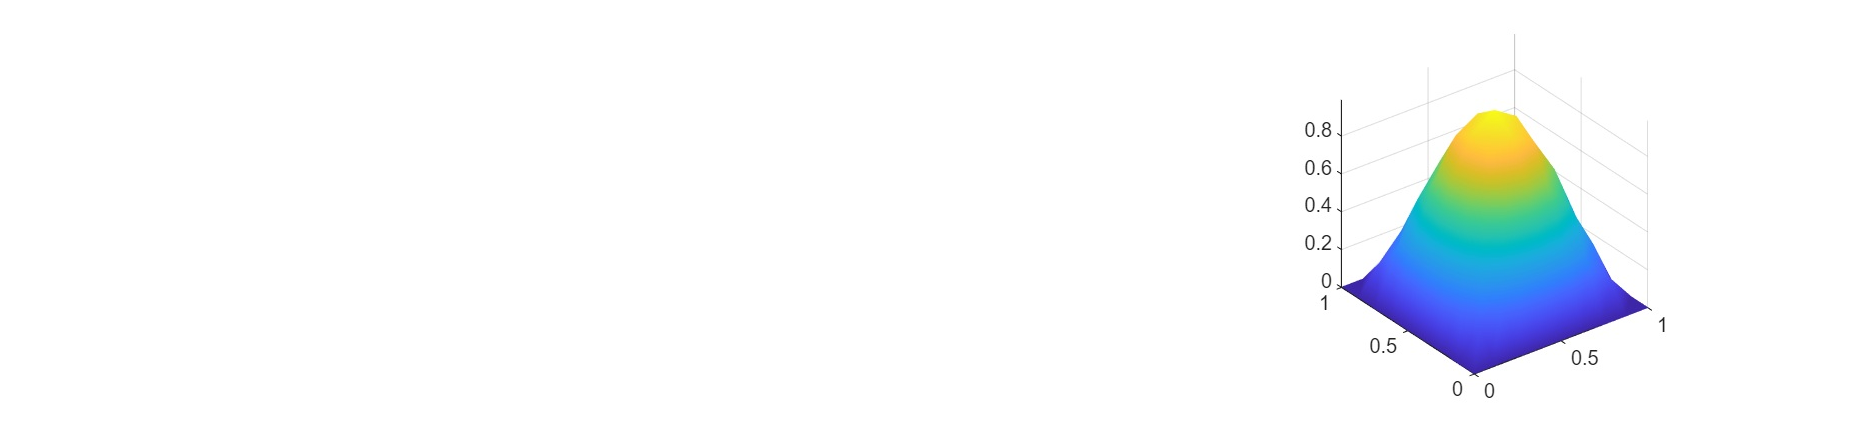
\includegraphics[width=\textwidth]
                            {../../Programming/Linear Finite Element Methods/image/pic2FEM_0.125.pdf}
                    \end{subfigure}
                    \caption{$h=0.125$ 时 $u_h$ 的图像}
                    \label{$h=0.125$ 时 $u_h$ 的图像}
                \end{figure}
    \item[(c)]  误差随网格尺寸变化的曲线如图 \ref{$H^1$ 范数下的误差}
                和图 \ref{$L^2$ 范数下的误差} 所示
                \begin{figure}[htbp]
                    \centering
                    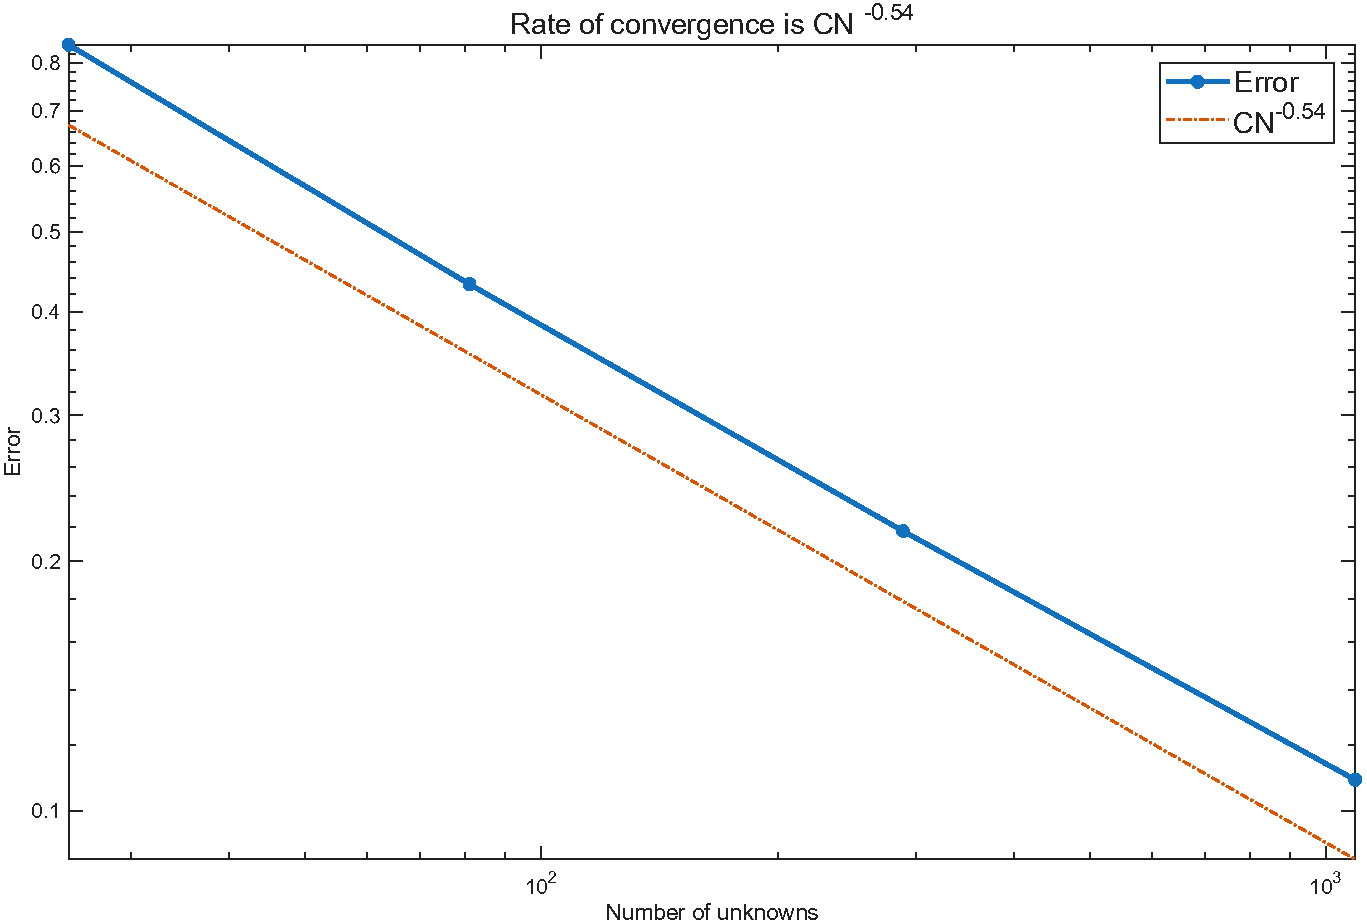
\includegraphics[width=0.8\textwidth]
                            {../../Programming/Linear Finite Element Methods/image/rateH1norm.pdf}
                    \caption{$H^1$ 范数下的误差}
                    \label{$H^1$ 范数下的误差}
                \end{figure}
                \begin{figure}[htbp]
                    \centering
                    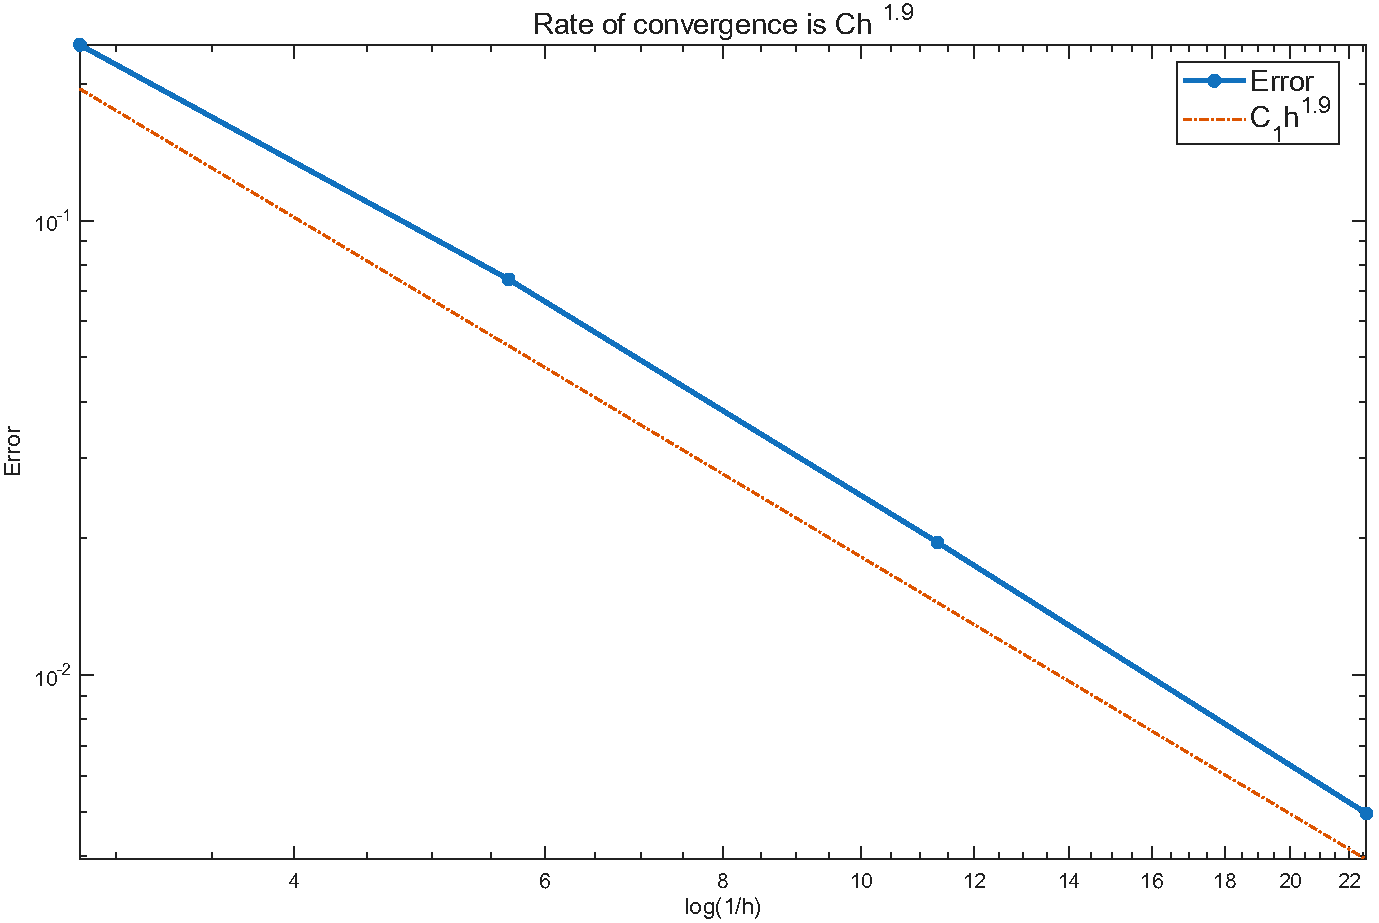
\includegraphics[width=0.8\textwidth]
                            {../../Programming/Linear Finite Element Methods/image/rateL2norm.pdf}
                    \caption{$L^2$ 范数下的误差}
                    \label{$L^2$ 范数下的误差}
                \end{figure}
\end{enumerate}

% ===============================================

\printbibliography

\end{document}